\documentclass{article}
\usepackage[utf8]{inputenc}

\usepackage{amssymb,amsmath,amsfonts,longtable,amsthm,
booktabs, comment,array, ifpdf, tabularx,url,color,array,colortbl,hyperref,graphicx, physics,siunitx}
\usepackage[hmargin=3cm,vmargin=3cm]{geometry}
\usepackage[]{algorithm2e}


\newtheorem{definition}{Definition}
\newtheorem{lemma}{Lemma}
\newtheorem{corollary}{Corollary}
\newtheorem{proposition}{Proposition}
\newtheorem{remark}{Remark}
\newtheorem{assumption}{Assumption}

\usepackage[normalem]{ulem}
\usepackage[capitalise]{cleveref}
\hypersetup{
    colorlinks=true,
    linkcolor=blue,
    filecolor=magenta,      
    urlcolor=blue,
    pdfpagemode=FullScreen,
}

\newcommand{\mary}[1]{ {\color{magenta} Mary:  #1 }}

\title{Not So Slo\sout{w}th:\\  Invertible VDF for Ethereum and others}
\author{Dmitry Khovratovich\\Ethereum Foundation \and Mary Maller\\Ethereum Foundation \and Pratyush Ranjan Tiwari\\Johns Hopkins University}


\begin{document}

\maketitle

\tableofcontents

\section{Introduction}

Many distributed protocols benefit not only from fast but also from (guaranteed) slow computations. 
When we say guaranteed slow computations we mean that there is a lower bound on the time the computation takes even if one has access to an unlimited number of cores i.e. the computation cannot be parallelized.
Slow computations are often required when a party is supposed to produce an output that will eventually benefit some other participants, so that the slowness of computation would guarantee unpredictability and thus fairness.

An example of this requirement in Ethereum 2.0 is the following. A group of 32 validators progressively builds a chain of collective randomness, also called a beacon chain, with one value $O$ generated per epoch $\mathcal{E}$. The value $O$ must be computed by the leading validator of $\mathcal{E}$ and must depend on certain inputs produced by other validators during $\mathcal{E}$. When generated, $O$ serves as the source of entropy in other chains and thus affect a number of computations potentially beneficial to the validator. It is thus of utmost importance to ensure that $O$ can be outputted only after a certain \emph{delay}. In other words, $O$ is derived from a \emph{verifiable delay function} (VDF).

A number of VDF constructions has been proposed in the recent past~\cite{DBLP:journals/ijact/LenstraW17,DBLP:conf/eurocrypt/Wesolowski19,DBLP:conf/crypto/BonehBBF18,DBLP:conf/innovations/Pietrzak19a} with their own advantages and limitations.
The VDF Alliance seeks for a concretely-efficient post-quantum VDF which may be used by L1 projects such as Cosmos, Ethereum, Filecoin, Tezos as well as L2 applications. The post-quantumness requirement rules out the promising RSA VDF~\cite{DBLP:conf/eurocrypt/Wesolowski19,DBLP:conf/innovations/Pietrzak19a}, but leaves open the possibility for VDFs based on verifiable computation, which are the subject of this report.

\section{Requirements}

On the high level, a protocol party, when outputting value $O$, also proves a statement of kind
$$
\text{I have spent at least $t$ time to produce }O.
$$
It is not important how exactly $O$ is computed but it \emph{is} important that the parameter $t$ be close, or at least  lower bound the actual time spent. The applications of VDF also yield separate requirements for hardware (where it is implemented), security properties, and statement parameters, which are all listed below.

\subsection{ Delay statements}

A delay statement is a statement of the form \begin{verbatim}
    delay(input, difficulty) == output
\end{verbatim} or equivalently
$$
F(I,d) = O
$$
where $I$ and $O$  are  integer (tuples)  and $d$  is a non-negative integer. The difficulty parameter regulates the execution time. We need certain delay granularity, i.e. the difficulty can vary with precision in seconds. This naturally suggests that $F$ is an iteration of some function $f$ with sufficient granularity. A single call to $f$ is then declared the unit of difficulty $d$, with $d\approx 2^{24}$ (for proposals listed in \cref{sec:proposal}) corresponding to 1 second. We restrict ourselves to delay statements with:
\begin{itemize}
    \item 15 sec to 3 days \textbf{delay range} ($2^{28}\leq d\leq 2^{42}$);
    \item  1 sec \textbf{delay granularity} --  ($d =0 \pmod{ 2^{24}}$).
\end{itemize}

\subsection{ Delay hardware}

The delay hardware is supposed to be a USB stick fitted with an ASIC implementing the VDF with  an additional requirement: every second an intermediate output   is streamed to the host in real time. As the  hardware is not yet manufactured, it can   be simulated by precomputing every about $2^{24}$-th round outputs and reading the appropriate output every $2^{24}\cdot 64$ ns $(\approx 1s)$.



\subsection{ Delay proofs}\label{sec:proofs}

Existing VDF constructions rely on a separate proof system that proves correctness of the VDF computation and thus ensures the delay statement. Clearly, the security of VDF relies on the one of the proof system.  The following requirements are given:
\begin{enumerate}
    \item First, a proof system should provide reasonable security level in a widely accepted security model. A random oracle model is chosen for its simplicity and versatility. There are two flavours of it:   \emph{programmable} and \emph{non-programmable ROM}. The former assumes we can dynamically select RO outputs in a simulation for the security proof, which simplifies the proof but formally contrasts with real-world instantiations of RO with hash functions, whose functionality is pre-fixed. The latter model is somewhat closer to the reality but such security proofs are not always available. We thus \emph{prefer}  the non-programmable ROM but it is not a strong requirement. Regarding the security level, at least 120 bits of security is required  (possibly under additional assumptions on some primitives used in the system).
    \item Secondly, a proof of a delay statement, should be \emph{post-quantum secure}.  Concretely, no quantum attacks should exist on underlying primitives, and additionally the security in the random oracle model, if being employed, should translate to quantum oracles. More precisely, at least 80 bits of \textbf{provable soundness in a quantum random oracle model} is required, with slight preference for non-programmable one.
    \mary{should the proof not be computable on a classical machine as well.}
    \item The proof should be \textbf{compact}. It is understood that the post-quantum security makes it difficult to be truly succinct (e.g. a few kilobytes), but it should be possible to contain the proof into 200 kBytes.
    \item The proof should be  verified within very short time (\textbf{succinct verification}). Concretely, we require at most 20ms verification time on a Raspberry Pi 4 Model B (single thread, no overclocking).
\end{enumerate}

\subsection{Cryptographic primitives and assumptions}
 
It is natural to accept widely used cryptographic primitives as secure ones. For instance standard hash functions such as SHA-256 and SHA-3 (Keccak)   may be assumed to be ideal 256-bit hash function and may be used to instantiate a 256-bit random oracle in the Fiat-Shamir transformation  and similar operations. 
It should be noted however that the regular hash functions are not well suited for most proof systems capable of proving delay statements. As a result, their usage in delay proofs is probably limited. 
%Further, random oracle queries heuristically instantiated by SHA256 calls may be arithmetised in a recursive verifier circuit, e.g. as done in [Halo Infinite](https://eprint.iacr.org/2020/1536.pdf). No other cryptographic assumption or heuristic may be used.
%\end{assumption} 



\subsection{ Prover hardware system}

We have a separate requirement to a potential  prover hardware system. We expect it to be a prover rig with prover software producing delay proofs for $1\leq u \leq 8$  always-active delay hardware units. The requirement is to design and implement a prover system with
\begin{itemize}
    \item  \textbf{Commodity hardware} -- the prover rig is built from off-the-shelf commodity hardware and requires little assembly;
 \item  \textbf{Low latency} -- delay proofs are produced with a latency (relative to the delay function output produced by the delay hardware) of:
 \begin{itemize}
     \item at most 10\% of the delay time if  $d\geq 2^{36}$ (i.e. more than an hour);
          \item at most 20\% of the delay time if  $d\geq 2^{32}$ (more than a few minutes);
               \item at most 40\% of the delay time if   $d \geq 2^{28}$ (all other cases);
 \end{itemize}
 \item \textbf{Permissive licensing} -- the prover software is open-sourced under the Apache 2.0 license.
\end{itemize}



\section{VDF definitions}

We start with recalling and adapting definitions of verifiable delay function protocol. 

\subsection{Generic VDF}\label{sec:genvdf}

Following the definition of VDF by~\cite{DBLP:conf/crypto/BonehBBF18} we consider only protocols of the following form:
\begin{itemize}
    \item The protocol is executed by calling some function $F$, which takes a long time;
    \item After $F$ finishes, one has to run another function $\Pi$ to produce a delay proof $\pi$.
\end{itemize}
We say that the protocol $(F,\Pi)$ is a \emph{verifiable delay function}  if it has the following features:
\begin{itemize}
    \item \textbf{Completeness:} Honest parties can execute it by calling $F$ in $t$ sequential steps and then by creating a proof $\pi$ that will be accepted by a verifier. It is ok if there is a non-zero, but from all points of view negligible, chance to fail to produce a proof, even though many practical VDF proposals do provide \emph{perfect completeness}, i.e. a proof can be always found.
    \item \textbf{Fast verification:} The proof $\pi$ can be verified in time polylogarithmic of $t$  (i.e. exponentially faster than the time needed for computation).  Note that this requirement rules out the designs based on computing an iterative function over a graph of a \href{https://cs.brown.edu/research/pubs/theses/ugrad/2019/zhang.aaron.pdf}{special form}, so that only a fraction of edges of the graph have to be proven, as these fractions turn to be bigger than polylogarithmic functions for practical parameters.
    \item \textbf{Non-malleability:} For any starting point $I$ and proof $\pi$ it should be difficult to find $(O'\neq O=F(I))$ that can be verified by $\pi$. Here by difficulty we mean only the complexity of the online phase, and may ignore (or take with a smaller factor) the cost of  precomputations.
    \item \textbf{Sequentiality or Delay:}  For any starting point $I$ it should be difficult to compute $(O,\pi)$ faster than in $\sigma t $ time for some  $\sigma $ close to 1. Note that we can allow asymptotically sublinear methods of computing as long as the constants are prohibitively large to be an actual time improvement.
\end{itemize}
It turns out that if we include quantum adversaries, then the only existing candidate is a combination of sequential algebraic transformation and a quantum-secure verifiable computation protocol. In order to boost the proof phase, the transformation $F$ is chosen to be invertible with low algebraic degree of the inverse. The entire construction is then called  \emph{invertible  VDF}.  

\subsection{VDF proofs based on Verifiable Computation}

Verifiable Computation (VC) schemes are a family of proof of knowledge protocols, where Prover convinces Verifier that $O$ is the result of program $P$ applied to some input $I$, so that it is impossible to craft a proof that would pass the verification without actually computing $O$ (= knowing all intermediate steps of computation). We see that this is exactly what is required for a delay proof, however, the existing VC schemes vary greatly in performance and requirements:
\begin{itemize}
    \item Scalability: Prover time can be linear or superlinear of actual execution time. Note that our requirements potentially allow for superlinear proofs as long as they can be parallelized enough to make the total latency only moderately smaller than the execution time (\cref{sec:proofs});
    \item Setup: A proof system may utilize a so called common/structured reference string (CRS/SRS) as a source of entropy and hidden secrets. As the creator of SRS is able to forge proofs, one has to run complicated multi-party ceremonies in order to share the secret   among participants and make no single party able to attack. Note that the size of CRS is usually proportional to the size of the computation (expressed as a circuit), so it can be very large for VDF. This makes us consider proof systems that do not require trusted setups~\cite{DBLP:conf/ccs/AmesHIV17,DBLP:conf/sp/WahbyTSTW18,DBLP:conf/sp/BunzBBPWM18,DBLP:conf/crypto/Ben-SassonBHR19} 
    \item Verifier scalability: with a few exceptions~\cite{DBLP:conf/sp/BunzBBPWM18}, the VC proof systems allow verifier to be sublinear, if not constant-time, of the computational time. For the application of VDF constant-time and logarithmic-time verifiers are allowed, but a lot depends on the constant factor in the latter case.
    \item Succinctness: Proof size can be constant-size, logarithmic of program length, or even larger. The constant-size proofs are usually possible only in proof systems with trusted setup, which we have ruled out. As a result, logarithmic-size proofs seem to be the only option. 
\end{itemize}

We expect that the delay function $F$ will be tailored to the specific choice of the VC proof system.

\subsection{ Invertible VDF }

In order to have delay granularity, it is convenient to have $F = f^D$ for some function $f$ (called \emph{base function}) and integer $D$ being a multiple of the granularity parameter (see \href{http://stevengoldfeder.com/papers/BGB17-IEEESB-proof_of_delay_ethereum.pdf}{also}). The reason is that the  VC proof systems typically define computation as an arithmetic circuit  with the statement of correctness being equivalent to a system of algebraic equations that relate intermediate steps of the computation. The cost of constructing a VC proof for VDF is determined by the degree of these equations, which is not always equal to the degree of $f$. Vice versa, we would be interested in function $f$ such that the degree of its inverse would be much smaller as this would reduce proportionally the time  needed to compute the proof $\pi$.

%Let $f(\mathbf{x})$ be a bijective function over $\mathbb{F}\approx Z_{N}$. The VDF proof is 
%a tuple $(I,O,\pi)$ which proves that $f^D(I)=O$. For $F = f^D$ to be a VDF the proof verification time should be logarithmic in $D$.

\begin{definition}
Let $\widehat{f}$ be the inverse of $f$. We say that $f$ is $\gamma$-invertible if the cost of $\widehat{f}$ is $\gamma$ times the cost of $f$. One-way functions over $Z_N$ are at most $N$-invertible.
\end{definition}


%**Definition**. The *inversion* problem for $F$ is to find $x$ for given $y$ such that $F(x)=y$.
\begin{remark}
By using invertible functions for $F$ we rule out the  Hellman time-memory tradeoff~\cite{DBLP:journals/tit/Hellman80}. The latter is a generic method to find a preimage for function $F(x)\rightarrow y$ assuming that the attacker can precompute $F$ on its entire domain (size of $N$) and store a certain part of this precomputation in the memory. The Hellman method tells us how to store these calls in the most efficient way so that a preimage to arbitrary $y$ can be found in less than $N$ calls. Clearly, this approach is not useful   for  invertible functions. 

\end{remark}

\subsection{Invertible VDF flow}

\cref{sec:genvdf} provides a generic description of a VDF, but leaves out a couple of subtle details. Concretely, we want to address the typical scenario that prover is not allowed to start the protocol at arbitrary moment, but rather he is given a seed or a family of possible seeds. In fact, the latter is more probable and we want to emphasize the fact that prover has enough freedom/entropy in selecting the seed so that he can even guess a valid seed with non-negligible probability. We capture this scenario by using an input predicate $\phi$, which is communicated to prover at the start of the protocol. However, the prover knows beforehand the fraction of possible inputs that $\phi $ will allow. For example, if a concrete application requires that invertible VDF is computed over $S_1||S_2$ where $S_1$ is given to the prover and $S_2$ is arbitrary then $\phi(I)=true$ iff $I$ starts with $S_1$. Such inputs are easy to enumerate. A more elaborate scenario is that the VDF is computed over $H(S_1||S_2)$ where $H$ is a preimage-resistant hash function.  In the latter case a Prover who does not know $S_1$ can't efficiently categorize his precomputations.


We thus suggest the following description:
\begin{enumerate}
    \item \textbf{Setup} -- Prover learns the input domain $\mathcal{W}$ and input density, i.e. the (approximate) fraction of elements $\mathcal{W}$ that can be selected as a seed.
    \item \textbf{Start} -- Prover is given \emph{ input predicate} $\phi$  over $\mathcal{W}$. 
    \item \textbf{Computation} -- Prover selects   $I$ such that $\phi(I)=true$. Then he computes $O=F(I)$.
    \item \textbf{Proof} -- if $\chi(O)=true$, Prover creates an IVC proof $\pi$ and submits $(I,O,\pi)$ to Verifier.
    \item \textbf{Verification} -- Verifier checks $\pi$.
    \item \textbf{Verification} -- Verifier checks $\pi$.
\end{enumerate} 
Note that $\phi$ is crucial, otherwise it is possible to pre-select a valid $O$, invert $F$ to some preimage $I$, and use it in further proofs.

Note that Prover can start computing the proof right after $\phi$ is known. However, he may spend some time selecting $I$ if this reduces the computational time or cost.

\begin{definition}
We say that the protocol \emph{allows grinding} if Prover is able to efficiently enumerate many $I$ such that
$\phi(I)=true$.
\end{definition}
 An example is when $I$ must be a hash of some preimage $I'$, with the hash function being finally determined only in the setup phase.


\subsection{ Sequentiality}

We would like to expand on the sequentiality property from \cref{sec:genvdf} so that we capture precomputations. Indeed, if Prover is able to precompute $F$ on the entire domain or a big fraction of it, and store the results in an efficiently accessible memory so that certain part of the \textbf{Computation} phase can be sped up, then the function is clearly unsuitable for a VDF.

\begin{definition}
The function $F$ is \emph{$(\alpha,\beta,M)$-sequential} if $M$ precomputation (calls to $F$) gives the chance $\alpha$ to reduce the running time of $F$ to $\beta$.

\end{definition}

In practice, we need that $F$ is $(\alpha,\beta,M)$-sequential for $\alpha$ and $\beta$ close to 1 and $M$ being the security level (in our case 128 bits).

As we consider security against quantum attacks, we should have an analog of sequentiality property for quantum machines.


\begin{definition}
The function $F$ is \emph{$(\alpha,\beta,M)$-quantum-sequential} if $M$ precomputation (quantum calls to $F$) gives the chance $\alpha$ to reduce the running time of $F$ to $\beta$.

\end{definition}


\section{  Attacks on invertible VDFs}

In this section we explore generic attack strategies that are applicable to all instances of invertible VDFs that we consider.

\subsection{  Precomputation attacks}\label{sec:precomp}

Here we consider attacks on sequentiality that arise from the ability of the attacker to precompute certain calls to $F$. Note that for the security level of 128 bits we allow an adversary to make $2^{128}$ precomputation calls to $F$. Recall that the VDF function $F$ maps $\mathcal{W}$ of size $N$ to itself.

\subsubsection{Attack 1}

The simplest attack works as follows:
\begin{enumerate}
    \item Apply $F^{-1}$ (i.e. invert $F$) to the entire domain $\mathcal{W}$  and create a proof for every inversion.
    \item Store results as $\overline{\mathcal{W}}=\{(I,O,\pi)\}$.
    \item When $\phi$ is known, find any $I\in\overline{\mathcal{W}}$ for which $\phi(I)=true$ and retrieve $(O,\pi)$ from $\overline{\mathcal{W}}$.
\end{enumerate}
This costs at most $\gamma N$ time and $N$ space. Thus any function is $(1,0,N)$-sequential.

\subsubsection{Attack 2}

The same attack but available to the adversary running the equivalent of only $M$ calls to $F$, works as follows:
\begin{enumerate}
    \item Apply $F^{-1}$ (i.e. invert $F$) to  $M/\gamma$ elements of  $\mathcal{W}$  and create a proof for every inversion.
    \item Store results as $\overline{\mathcal{W}}=\{(I,O,\pi)\}$.
    \item When $\phi$ is known, check if there is $I$ such that  $(I,*,*)\in\overline{\mathcal{W}}$ and $\phi(I)=true$. If found then retrieve $(O,\pi)$ from $\overline{\mathcal{W}}$.
\end{enumerate}
This costs at most $M$ time and $M/\gamma$ space, but the chance to find the right $I$ is at most $\frac{M|\phi|}{\gamma N}$ with $|\phi|$ being the number of $I$ for which $\phi(I)$ is true, so that the function is $(\frac{M|\phi|}{\gamma N},0,M)$-sequential. If $\phi$ is chosen so that it is not trivial to find the intersection of $\overline{\mathcal{W}}$ and $|\phi|$, and one has to check each entry of $\overline{\mathcal{W}}$ separately, then the chance to find the right $I$ is only $\frac{GM}{\gamma N}$ where $G$ is the number of calls to $\phi$ that are made by the adversary (possibly in parallel) during the time required by application to compute VDF. In this scenario the VDF is at best is $$
(\frac{GM}{\gamma N},0,M)\text{-sequential}.
$$

Example 1: suppose   $M=2^{64}$, $G=2^{58}$, $N=2^{128}$, $\gamma=1/64$. Then an adversary who spends time equivalent to $2^{64}$ VDF forward precomputations, can compute the $F$ output after trying $2^{58}$  values for $\phi$.


\subsubsection{Attack 3}\label{sec:att3}

Another modification of the same attack\footnote{Suggested to us by Avihu Levi} works as follows:
\begin{enumerate}
    \item Compute not the full $F^{-1} = f^{-D}$ but the reduced version $f^{ \delta D}$, i.e. compute chains of length $ \delta D$ for some $\delta>0$ (and parts of future proofs if possible). In total it is possible to compute $\frac{M}{\gamma \delta}$ chains.
    \item Store results as $\overline{\mathcal{W}}=\{(I',O')\}$.
    \item When $\phi$ is known, select up to $G$ different values  $I$ such that $\phi(I)=true$ and start computing. For each intermediate call to $f$ check if the state matches any of $\overline{\mathcal{W}}$. If found then use the entry to reduce the computing time by the factor $ \delta$.
\end{enumerate}
The chance to meet a precomputed chain in the online phase is $\frac{(1-\delta)DGM}{ \delta\gamma N}$, so $F$ is at best
$$
\left(\frac{(1-\delta)DGM}{ \delta\gamma N},1-\delta,M\right)\text{-sequential.}
$$
 Note that this attack equally works for $F$ where each $f$ call is different. In this case each precomputation chain simply starts from a valid output state.



Example 2: suppose $D=2^{40}$, $M=2^{64}$, $N=2^{128}$, $\gamma=1/64$, $\delta=1/2$. Then an adversary who spends time equivalent to $2^{64}$ VDF forward precomputations, can compute VDF in $1/2$ of required time if he can compute $2^{18}$ VDF chains in parallel.


\subsubsection{Mitigation and parameter selection}\label{sec:mitig}

Looking at the sequentiality parameters, it is easy to see that the attacks get non-negligible probability to succeed whenever  $GM$ approaches $N/D$ where $G$ is the amount of computation spent in the online phase, $M$ is the amount of precomputation, and $D$ is the VDF difficulty parameter. Therefore it is natural to increase $N$ to mitigate it, for example to make $N = M^{1.5}$ (a bit risky)
 or $N=M^2$ or even bigger.  Assuming $G<M$ we can state that the security level of invertible VDF is roughly given by the value $\sqrt{N/D}$:
 \begin{equation}\label{eq:level}
     \text{Security level (VDF) }\approx \sqrt{\frac{N}{D}} \end{equation}
     Thus, in order to have 100 bits of security we need a 256-bit long $N$. 
 
 It is also clear that a simple $\phi$ also makes the attack easier. Thus we suggest using a preimage-resistant hash function as part of $\phi$, but not part of the proof. There can be many possible such $\phi$, and we suggest the already mentioned 
\begin{equation}
    \label{eq:phi}
    \phi_{S_1}(I) = true\;\Leftrightarrow\; \exists S_2:\,H(S_1||S_2)=I
\end{equation}
where $H$ is a regular cryptographic hash function (such as SHA-3) and $S_1$ is the parameter selected at the \textbf{Start} phase.

The ability to check sufficiently many different $S_2$ is also called \emph{grinding}. In the further analysis we always assume that it is possible to grind up to $2^{64}$ different inputs; if this is not the case in some application, the protocol is even more secure. 
 


\subsection{Grobner Basis and Algebraic}
This class of attacks exploits the algebraic nature of an invertible VDF.
Consider the reduced  $F$ as $F' = f^d$ for some $d<D$. If it is possible to solve the equation
\begin{equation}\label{eq:fd}
\widehat{f}^d(I) = O
\end{equation}
where $O$ is known and $X$ is unknown, then one can run the equation solver instead of applying $f^d$. This attack only succeeds if \eqref{eq:fd} can be solved fast then running $f^d$. 

If \eqref{eq:fd} is multivariate, then the best generic technique is applying Groebner basis algorithms~\cite{DBLP:books/daglib/0091062,faugere2002new}. These algorithms find a generating set for the ideal generated by \eqref{eq:fd} so that they can be solved as univariate equations. Little is known about the actual complexity of Groebner basis algorithms, but the available heuristic analysis suggests that it is exponential in $d$, thus quickly become impractical. Even in the unlucky case when a Groebner basis can be found for the system of equations that describe a VDF, we still face the problem of solving univariate equations for it.

Univariate equations over finite fields can be solved using Berlekamp or  Cantor-Zassenhaus algorithms. It is known~\cite{cantor1981new} that an equation of degree $r$ can be solved using $O(r^3\log p )$ operations over elements of $\mathbb{F}_p$. This should be compared with $O(d\log p)$  operations needed to compute $f^d$. We conclude that, unless $f^d$ has some structure that makes the univariate equations of its Groebner basis of very low degree (at most $\sqrt[3]{d}$), generic algebraic methods are not applicable even if $f$ or $\widehat{f}$ has univariate representation.

\section{ Quantum algorithms}

Quantum algorithms are the algortihms specially designed for quantum computers. A unique property of a quantum computer is  able to perform  operations not on a single state but on   a superposition of states, so that certain classical algorithms can be amortized. The most famous examples are Shor's algorithm for factorization~\cite{DBLP:conf/focs/Shor94}
and its derivative for discrete logarithm search, as well as the Grover search algorithm~\cite{DBLP:conf/stoc/Grover96}. The latter is our main interest as we have excluded factoring- and DLP-based schemes from consideration.

\subsection{Grover's algorithm}

The Grover algorithm was originally formulated as a database search, however, it can be equivalently written as a preimage search algorithm for some hard-to-invert function.  Concretely, given $O\in Z_N$ (or any other domain efficiently mappable to $Z_N$) and function $H$, Grover algorithm finds $I$ such that $H(I)=O$ in time equivalent to $\sqrt{N}$ calls to $H$ on a quantum computer. Note that the algorithm is inherently sequential and so far no one knows how to parallelize it so that the computing time can be reduced. The probability to find the preimage in $t$ time grows as $t^2/N$~\cite{DBLP:journals/sigact/BrassardHT97}.

\subsubsection{Single-target Grover's}

Grover's algorithm makes a particular sequence of operations multiple times. At a high-level, after each iteration the probability amplitude of the marked index state is increased. Once enough iterations are performed, this amplitude is high enough that when a measurement is performed, with high probability the resulting index corresponds to the special marked state. Each iteration is made of 2 simple operations. The following description assumes that we are using Grover's algorithm to perform unstructured search on a boolean function $f: \{0, 1\}^n \rightarrow \{0, 1\}$ where there is only one unique element $x^\prime$ such that $f(x^\prime) = 1$ and $N = 2^n$. The input to Grover's algorithm is an equal superposition of all inputs:

$$ \phi_0 = \frac{1}{\sqrt{N}}\sum_{x=0}^{N-1} \ket{x} $$

The 2 operations performed at each iteration of Grover's algorithm are as follows:

\begin{itemize}
    \item \textbf{Amplitude flip} $\ket{x^\prime} \rightarrow -\ket{x^\prime}$: The amplitude of the unique element $x^\prime$ is negated. This operation is implemented using the following gate logic:
    
    $$ (-1)^{f(x)}\ket{x}=\left\{\begin{array}{ll}
\ket{x} & \text { if } f(x)=0 \\
-\ket{x} & \text { if } f(x)=1
\end{array}\right.  $$
    
    Post this operation, the state of the input qubits is:
    
    $$ -\frac{1}{\sqrt{N}}\ket{x^\prime} + \sum_{x \neq x^\prime} \frac{1}{\sqrt{N}}\ket{x} $$
    
    \item \textbf{Diffusion operator}: The goal of the diffusion operator is to increase the amplitude of $x^\prime$. The diffusion operator flips the amplitude of each $x \in \{0, 1\}^n$ around the average amplitude $\mu = \frac{1}{N}\sum_{x} A_x$ where $A_x$ represents the amplitude of $x$. This operation is implemented using the following gate logic:
    
    $$ \sum_{x \in\{0,1\}} \alpha_{x} \ket{x} \mapsto \sum_{x \in\{0,1\}^{n}}\left(2 \mu-A_{x}\right) \ket{x} $$
    
    The mean amplitude before the diffusion operator is roughly $\frac{1}{\sqrt{N}}$. Therefore, after the diffusion operator all entries remain roughly the same as they go from, $\frac{1}{\sqrt{N}}$ to $\frac{2}{\sqrt{N}} - \frac{1}{\sqrt{N}}$. However, the amplitude of $x^\prime$ , $A_{x^\prime}$, goes from $-\frac{1}{\sqrt{N}}$ to $\frac{3}{\sqrt{N}}$.
    
\end{itemize}

The above two operations are then repeatedly applied, increasing the amplitude of $x^\prime$ after each round by $\frac{2}{\sqrt{N}}$. After $O(\sqrt{N})$ rounds, the amplitude of $x^\prime$ is up to a desirable constant and at this point a measurement is performed which collapses the state to $x^\prime$ with constant probability.

\subsubsection{Multi-target Grover's}


For us the main interest is the multi-target version of the Grover algorithm, which we hope to use in the pre-computation attacks. The same algorithm works in the multi-target case but now instead of requiring $O(\sqrt{N})$ iterations, the number of iterations required is $O(\sqrt{\frac{N}{k}})$ as there are $k$ targets whose amplitude gets amplified after each iteration. %\textbf{\textit{(Should we consider the case when $k$ is unknown?)}} 
Hence, the multi-target Grover's finds a pre-image  to one of $k$ targets in time $\sqrt{N/k}$. The probability to find the pre-image in $t$ time grows as 
\begin{equation}
    \label{eq:mt-grover}
    f_{MG}(k,t,N) = kt^2/N
\end{equation}according to \cite{Brassard_2002}.

\subsubsection{Quantum Parallelism}

Achieving speed-ups via parallelism is an important line of work for most search algorithms. However, in the case of Grover's algorithm, the work of Zalka~\cite{Zalka_1999} proves that quantum searching can not be parallelized better than the naive case. The naive case assigns different parts of the search space to separate quantum computers. And hence, you get a linear improvement in search time with multiple quantum computers corresponding to increased computational cost. 

\subsection{Attacks based on Grover's}

\subsubsection{Grover Attacks 1 and 2}

We can apply Grover algorithm to our precomputation attacks from \cref{sec:precomp}. 
The first two attacks work as follows:
\begin{enumerate}
    \item Apply $F^{-1}$ (i.e. invert $F$) to  $M/\gamma$ elements of  $\mathcal{W}$  and create a proof for every inversion.
    \item Store results as $\overline{\mathcal{W}}=\{(I,O,\pi)\}$.
    \item When $\phi$ is known, check (using Grover) if there is $I$ such that  $(I,*,*)\in\overline{\mathcal{W}}$ and $\phi(I)=true$. If found then retrieve $(O,\pi)$ from $\overline{\mathcal{W}}$.
\end{enumerate}
The improvement comes in the setting when finding the right $I$ is not easy i.e. when we have to check each $\phi(I)=true$ individually. We run Grover algorithm on the set $\overline{\mathcal{W}}$ of targets in the Computation phase, and in order to increase the attack probability we run several (denoted by $G$) copies of Grover in parallel. Let us assume that a call to $\phi$ costs as much as a call to $f$. Then if each Grover is run for $\beta D$, then the chance to match any element of   $\overline{\mathcal{W}}$ can be derived from \eqref{eq:mt-grover} as 
\begin{equation}\label{eq:pmg}
    P_{MG}(\beta, D,N) = \frac{\beta^2 G D^2M}{\gamma N}
\end{equation}
so that the VDF protocol is
$$
\left(\frac{\beta^2 G D^2M}{\gamma N},\beta,M\right)\text{-quantum-sequential}
$$

Example 3: suppose   $M=2^{64}$, $D=2^{40}$, $N=2^{192}$, $G=2^{40}$, $\gamma=1/64$. Then an adversary who precomputes an  equivalent of $2^{64}$ VDF forward precomputations, can compute the $F$ output in  $1/2$ time using $2^{40}$ instances of Grover algorithm with probability $1/4$.




\subsubsection{Attacks that do not work}

Interestingly, Grover algorithm does not  seem  to improve if we switch from attacks 1-2 to   the chain-based approach (\cref{sec:att3}). The reason is that the   latter requires to compute several iterations of $f$ which can not be iterated in Grover. Thus we conclude that \eqref{eq:pmg} is the best we can hope with Grover.

For the same reason we can not effectively run a quantum meet-in-the-middle attack~\cite{DBLP:journals/sigact/BrassardHT97} on $F$ by splitting in two parts, as Grover would need to compute many iterations of $F$ sequentially.

We conclude that the security level of invertible VDFs against quantum adversaries is given by the formula
 \begin{equation}\label{eq:level2}
     \text{Security level (VDF) }\approx {\frac{\sqrt{N}}{D}} \end{equation}
which is only by the factor of $\sqrt{D}$ lower than the classical one \eqref{eq:level}.


\subsection{Practicality of Quantum Search}

Grover's search is usually discussed for some oracle function $f(\cdot)$. However, several practical issues need to be considered when a specific construction of $f(\cdot)$ is being considered. The work of Viamontes, Markov and Hayes~\cite{practicalityGrover05} focuses on these issues.  The first issue is that in order to query $f(\cdot)$ in superposition, we need a quantum hardware implementation of  $f(\cdot)$. While a quantum circuit is usually similar in size to its classical counterpart, if the the circuit's maximum depth exceeds $\sqrt{N}$ then the evaluation of  $f(\cdot)$ is the more cost consuming part of searching a size $N$ database. This would diminish the quantum speedup by a considerable amount. Hence, to come up with resource estimates for quantum attacks we first come up with the quantum circuits for the VDF candidates. 


\subsection{Quantum Grobner}

We note that quite little is known about the quantum complexity of Groebner basis algorithms nor of the equation solving. There exist several results showing that Gaussian elimination of sparse matrices can be sped up greatly on a quantum computer\url{https://arxiv.org/abs/0811.3171}, which in turns would shorten the elimination step in the Groebner basis algorithms. However, it is the subject of the future research if an algorithm like F4 or F5~\cite{faugere2002new} can be improved as a whole. We expect that if it can be done, running a quantum algorithm every few steps would induce high latency, and the high value of $D$ would rule out such strategies. To the best of our knowledge there is no quantum improvement to solving univariate equations either.
 
\section{Quantum Circuits for VDF candidates}
 
Quantum circuits for the VDF candidates are required for a proper estimation of resources required to carry out any quantum attacks. Previous work~\cite{estimatesQuantumAES} on quantum resource estimation follows a similar approach. While attack resource estimation might focus on restricting the number of qubits~\cite{estimatesQuantumAES} or restricting circuit depth~\cite{keysearchQuantumAES}, studying the quantum circuits is the clear first step in any case. The higher level goal is to construct a circuit $\mathcal{C}$ for each of the VDF candidate functions, to implement the operation $\ket{I}\ket{0} \mapsto \ket{I}\ket{VDF_I(x)}$. 

To design the quantum circuits we look at the basic operations utilized in all of the candidates. Quantum gates for performing addition, multiplication, square-root and cube-root calculation in finite fields are required as building blocks to construct the circuits. The work of Beauregard, Brassard and Fernandez~\cite{quantumArithmetic} gives us the circuits for addition and multiplication in a finite field. For the other operations we use these circuits as building blocks and construct them ourselves.

\subsection{Gates for Finite Field Arithmetic}

We are working in finite field $\mathbb{F}_p$ where the prime $p$ is $n$-bits long:

\begin{itemize}
    \item \textbf{Addition.} For the quantum circuit for addition in field $\mathbb{F}_p$, first a simple adder gate for integers is built. This allows adding a classical value to a quantum register. One way to do this is to take the quantum Fourier transform (QFT) of some qubit register $\ket{x}$ to the QFT of the sum $x + a$. This is called the $\phi$-adder and was introduced by Gossett~\cite{quantumCarrySave}. The other method to construct this integer adder is via the carry-sum adder of Vedral, Barenco and Ekert~\cite{Vedral_Barenco_Ekert_1996}, which is similar to classical bit-wise addition. Once we have this integer adder, to build the adder gate for $\mathbb{F}_p$ we introduce control qubits. After addition of $a$, $p$ is subtracted for the register and then we access the most significant qubit of the register to check for an overflow. Using the QFT-based $\phi$-adder method requires $O(n^2)$ elementary gates in depth $O(n)$ on an $(n+1)$-qubit register. The constants considering the elementary gates complexity are small ($<10$). The carry-sum adder requires $O(n)$ elementary gates in depth $O(n)$ and needs $2n$ qubits.  Adding the control qubits bumps up the number of qubits required by a small constant. 

\item \textbf{Multiplication.} The quantum circuit for multiplication in field $\mathbb{F}_p$ utilizes the addition gate above and uses a few control qubits to get the desired product. We skip the detailed description for brevity. If the QFT-based $\phi$-adder are utilized then multiplication requires $O(n^3)$ elementary gates in depth $O(n^2)$ on $(2n+3)$-qubits. However, if the carry-sum adder is used instead then we need $O(n^2)$ elementary gates in depth $O(n^2)$ working over $3n+2$ qubits. Once we have a multiplication circuit, exponentiation to power $\rho$ requires $O(\log \rho)$ multiplications via repeated squaring.


\item \textbf{Square-root calculation.} Previous work does not consider constructing a quantum circuit for square-root calculation over finite fields. Hence, our approach is to use the above gates as building blocks along with known classical algorithms. The Tonelli-Shanks algorithm~\cite{Shanks} is used classically to determine square roots in finite fields. However, this algorithm is randomized. The randomized part of Tonelli-Shanks finds a non-residue $D$ mod $p$. To make this calculation deterministic, this non-residue can be calculated once offline. Once $D$ is known, the algorithm is deterministic. Tonelli-Shanks algorithm~\cite{Shanks} works as follows. Let $x$ be a solution to $x^2 \equiv a \text{ (mod } p)$. The term $p-1$ is represented as $Q\cdot2^{s}$ where $Q$ is odd. Such a representation can easily be found by repeated division by $2$. The square-root $x$ can be followed using the following loop:

\begin{enumerate}
    \item Set $t = a^{(Q + 1)/2}$ and find the least $i$ such that $r^{2^i} \equiv 1 \text{ (mod } p)$ for $r = a^Q \text{ (mod } p)$.
    
    \item If $i=0$ then the square-root is $x \equiv \pm t \text{ (mod } p)$ otherwise set $y \equiv D^{Q(2^{s-i-1})} \text{ (mod } p)$ and repeat step (1) with $t = ty$ and $r = ry^2$
\end{enumerate}

We can construct a quantum circuit for performing these operations above as we can already perform finite field arithmetic. The pre-computed values can be input to the circuit. Other than non-residue $D$, inverse of $2$ can also be input as a pre-computed value to aid in finding the representation of $p-1$ as $Q\cdot2^{s}$. Overall, if a non-residue is given as input, Tonelli-Shanks algorithm runs in $O(\log^2 p) = O(n^2)$ time. Since the values of $t$, $r$, $y$, $D$ and $Q$ are essential for this algorithm, they will be stored in quantum registers. Moreover, each iteration requires two exponentiations to (at least) $Q$, the overall resources would consist of $O(n)$ qubits with small constants and at least $O(\log Q)$ multiplications. Therefore, calculating square roots requires roughly $4n$ qubits to store values, and $3n + 2$ qubits for multiplication. Since these estimates are lenient, we estimate one square-root calculation to require $\approx 10n$ qubits and $O(n^2)$ elementary gates in depth $O(n^3)$.

\item \textbf{Cube-root calculation.} Cube-roots can be calculated by just exponentiating to $p+1/3$. This requires $\log(p+1/3) \approx n$ multiplications. However, since the qubits can be reused, the number of qubits required to calculate cube-roots is the same as multiplication. However, the circuit depth required increases by a linear factor over the multiplication circuit.

\end{itemize}

\subsection{Resource Estimation}

An adversary aiming to mount a quantum attack on these VDF candidates would first need to design a quantum circuit implementing one round of the candidate functions. Such an adversary will try to minimize the number of qubits required to mount such an attack as that is one of the most expensive resource. In such a scenario, it might not be feasible to attack constructions that involve square-root calculation in a finite-field. 
\begin{table}[ht]
\caption{Arithmetic operations for a one round quantum circuit for VDF candidates}
\centering
  \begin{tabular}{|l | l | l | l| l|}
    \hline
     Candidates  & Additions & Multiplication & Square-root calculation & Cube-root calculation\\
    \hline
    MinRoot     & 3 & 0 & 0 & 1 \\
    VeeDo       & 4 & 2 & 0 & 2 \\
    Sloth++     & 4 & 0 & 2 & 0\\
    MinRoot Lite    & 4 & 0 & 0 & 1\\
    \hline
  \end{tabular}
  \label{Tab:Tcr}
\end{table}

We now estimate the concrete resource requirements for a quantum adversary to implement VDF candidates. This gives us a lower bound for the quantum resources required to mount any attack. Note that any search method would require it's own resources, over the resources required below. This gives us a way to determine the right VDF challenge difficulty over the years as quantum computers become more powerful and efficient. As is clear from Table 2, all VDF candidates are practically safe even if a $1000$-qubit quantum computer exists when $n = 128$-bits. For reference, the current best quantum computer in practice hasn't even reached $100$-qubits~\cite{}.

\begin{table}[ht]
\caption{Resource estimation for quantum circuits for 1-round VDF calculation}
\centering
  \begin{tabular}{|l | l | l | l| l|}
    \hline
     Candidates  & No. of Qubits ($q$) & Elementary Gates & Circuit Depth \\
    \hline
    MinRoot     & $q <10n$ & $O(n^2)$ & $O(n^3)$ \\
    VeeDo       & $10n < q <20n$ & $O(n^2)$ & $O(n^3)$ \\
    Sloth++     & $20n< q <30n$ & $O(n^2)$ & $O(n^3)$ \\
    MinRoot Lite    & $q \approx 10n$ & $O(n^2)$ & $O(n^3)$ \\
    \hline
  \end{tabular}
  \label{Tab:Tcr}
\end{table}

\section{Other attacks}


\subsection{MIMC reduction}

Here we provide an observation that relates the sequentiality of invertible VDFs to the security of some well-known symmetric key primitives. For this we recall the MiMC bijective transformation over $\mathbb{F}_p^2$ ~\cite{DBLP:conf/asiacrypt/Albrecht0R0T16}:
\begin{itemize}
\item Input $(x,y)\in\mathbb{F}_p^2$
    \item For $1\leq i \leq R$ repeat:
    \begin{enumerate}
        \item $(x,y)\leftarrow (y+x^3+c_i,x)$ where $c_i$ is a public constant that depends on $i$. In a keyed version, a key is also added $\bmod{p}$ with $c_i$.
    \end{enumerate}
\end{itemize}
The security of MiMC is based on the assumption that the resulting polynomial has large algebraic degree and it has no compact representation.
Despute the years of public scrutiny~\cite{DBLP:conf/asiacrypt/AlbrechtC0KLRS19,DBLP:conf/asiacrypt/Eichlseder0LORS20}, no counterargument to this assumption was found\footnote{There are certain cryptanalytic results for the binary field case and in the related key scenario, but they are irrelevant for our purpose.}. Computing Groebner basis has proven useless either. This hints that as long as the function $f$ in the VDF design resembles that of MiMC, we should expect little to no algebraic structure in the polynomial describing the iteration of multiple rounds, which in turn implies that these polynomials are kind of ``generic'' and ``random-looking''. Thus intuitively there should be no sequentiality shortcut as it should not be for random functions. 


We note that this argument holds as long as the polynomial describing the iteration has degree 3. It is known that certain quadratic polynomials yield short cycles and thus should not be used\cite{DBLP:journals/dm/VasigaS04}.



\subsection{Attacks on Verifiable Computation}

In this report we mostly ignore potential attacks on the proof system used in verifiable computation systems. We only note that they largely split into two groups: ones whose security is based on the hardness of discrete logarithm in elliptic curve or integer groups (and thus almost universally quantum insecure), and the ones that require little to no such assumption. However, not all protocols from the latter group have claimed post-quantum security as some of their components such as Fiat-Shamir challenge derivation are not proven post-quantum secure. We thus urge that in order to achieve post-quantum security it is desirable to use only those VC systems that do claim it (even though no formal proof of security may be given).

\subsection{Attacks on cube-root-based candidates}

Cube-root is considered as a possible sub-operation in some VDF candidates. We make the key observation that while operating on BLS/BN curves, the cube-root is not an injective function. Due to this observation, we can carry out the following attack to find collisions on cube-root based VDF candidates. 

The VDF input is the cryptographic hash of the seed. Given the hash of the seed, at each step, the output could be forked by finding 2 different inputs such that their cube-root is the same. Doing this is quite simple, let $x = y^3$ and let $w^3 = 1$, $w$ is a cubic-root of unity. Now clearly, $(yw)^3 = x$ could provide us with a valid collision. Assuming the function is applied for $n$ rounds. We could have upto $2^n$ inputs such that they all have the same VDF output. An adversary could use pre-processing to have with it a table to efficiently find a seed which maps to one of the collision inputs under the hash function.


\section{Concrete Proposals}\label{sec:proposal}

All proposals are considered in two settings: 128-bit field and 256-bit field, commonly denoted $\mathbb{F}_p$.

\subsection{Recommendations for $\phi$}

One can note that some VDF proposals employ a hash function at the first step of the computation, i.e. as part of $\phi$ in our terminology, whereas others do not. We have explained in \cref{sec:mitig} that the use of hash function makes all precomputation attacks universally harder, whereas it costs little for prover and verifier. We thus include it into our proposal (MinRoot) and advise all others do the same.

\subsection{MinRoot  (Khovratovich-Feist)}

\mary{Problem: need that p = 2 mod 3 for the cube root to exist.  This is not true e.g. if p = the order of BLS12-381.
Can it work e.g. taking 5th roots rather than cube roots?
}
For our proposal MinRoot we select function $f$ as part of $F$ so that the inverse $\widehat{f}$ is fastest possible to compute in the proof creation part. Concretely, we consider function $h(x) = x^{(2p-1)/3}$, which is the inverse of a cubic (i.e. low degree) function: $h^3(x) = x^{2p-1} = x\bmod{p}$. Then we define

\begin{enumerate}
    \item Input predicate $\phi$: $x_1$ is the seed, input is $I=(x_1,y_1)$, and the relation is $\phi(x_1,y_1)=true\leftrightarrow y_1=H(x_1))$ where $H$ is SHA-3.
    \item Computation: repeat for $1\leq i\leq D$
    $$
    (x_{i+1},y_{i+1}) \leftarrow   ((x_i+y_i)^{(2p-1)/3},x_i)+(0,i)
    $$
    \item Output $O = (x_{D+1},y_{D+1})$.
    \item Proof: create a VC proof (presumably STARK-based) that  $F(I) = O$.
\end{enumerate}

We aim for the performance here: at each step we make one exponentiation, and those are sequential.

MinRoot claims 128-bit security for 256-bit primes.

\begin{figure}
    \centering
    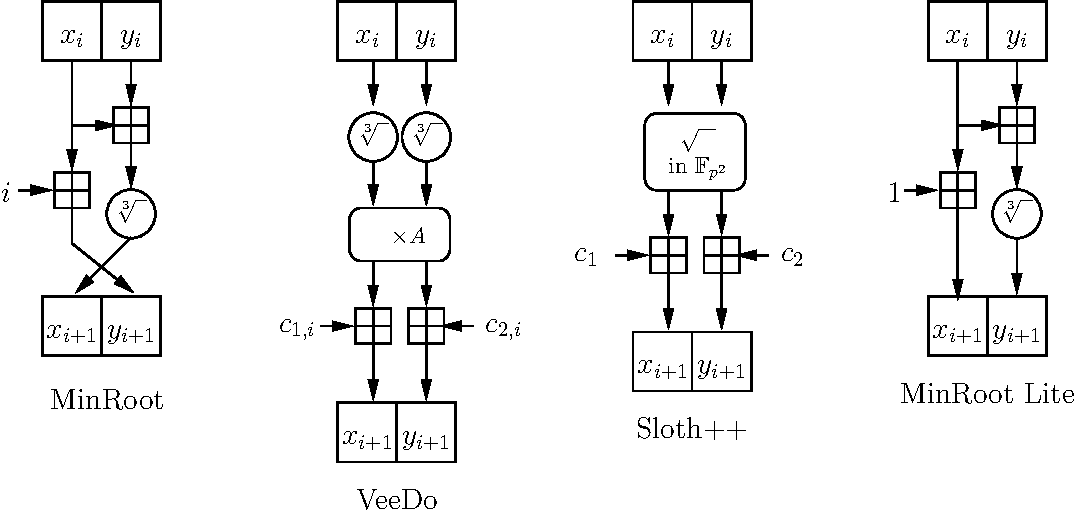
\includegraphics[width=10cm]{pics/mrsmall.pdf}
    \caption{One round of MinRoot and MinRoot Lite}
    \label{fig:mrl}
\end{figure}


\subsection{VeeDo (StarkWare)}

The VeeDo function is also based on the cubic roots in $\mathbb{F}_p$:
\begin{enumerate}
    \item Input predicate $\phi$: $x_1$ is the seed, input is $I=(x_1,y_1)$, and the relation is $\phi(x_1,y_1)=true\leftrightarrow y_1=x_1$.
    \item Computation: repeat for $1\leq i\leq D$
    $$
    (x_{i+1},y_{i+1}) \leftarrow A \cdot (x_i^{(2p-1)/3},y_i^{(2p-1)/3})+(c_{1,i},c_{2,i})
    $$
    where $A$ is an invertible matrix and $\{c_{1,*},c_{2,*}$ are some public constants.
     \item Output $O = (x_{D+1},y_{D+1})$.
    \item Proof: create a VC proof (presumably STARK-based~\cite{DBLP:conf/crypto/Ben-SassonBHR19}) that  $F(I) = O$.
\end{enumerate}
The difference to MinRoot is that a combination of a power function and the state swap is replaced with a full-blown affine transformation. This approach, well known in the theory of block cipher design, is supposed to  provide faster diffusion and to ease analysis. However, we note that the diffusion speed is not as important for our setting as sequentiality is, since after $2^{20}$ or more iterations the diffusion becomes almost perfect anyway. Regarding sequentiality, we remark that VeeDo spends two parallelizable exponentiations per round, whereas MinRoot does only one.  Thus for the same delay time and same state size VeeDo requires twice bigger hardware, whereas the smaller state would reduce the security. The same ratio holds for the proof size and computation time. We thus conclude that VeeDo is slightly inferiour to MinRoot

\subsection{Sloth and Sloth++ (Wesolowski-Boneh et al.)}
Sloth was suggested in~\cite{DBLP:journals/ijact/LenstraW17}. For the  $k$-bit a security level we select  a prime $p$ so that $p=4q+3$ for some $q$ and $p>2^{2k}$. Let $H$ be a regular cryptographic hash function such as SHA-2 with $2k$-bit output. The algorithm is as follows:
\begin{enumerate}
    \item Input predicate $\phi$: $x_1$ is the seed, input is $I=(x_1,y_1)$, and the relation is $\phi(x_1,y_1)=true\Leftrightarrow y_1=H(x_1)$.
    \item Computation: repeat for $1\leq i\leq D$
    $$
    y_{i+1} \leftarrow (\delta\sigma(y_i))^{(p+1)/4}\in\mathbb{F}_p
    $$
    where  $\sigma $ is a not fully specified ``simple'' invertible function such as bit permutation, and $\delta\in\{1,-1\}$ is chosen so that the result is quadratic residue.
 \item Output $O = y_{D+1}$. %$(H(H(s)),H(w),w)$
    \item Proof: direct evaluation of the inverse function.
\end{enumerate}



Boneh et al suggested in~\cite{DBLP:conf/crypto/BonehBBF18} a version more suitable for verifiable computation proofs. It is called  Sloth++ and it operates similarly over $\mathbb{F}_{p^2}$:
\begin{enumerate}
    \item Input predicate $\phi$: $s$ is the seed, input is $I=(s,x_1,y_1)$, and the relation is $\phi(s,x_1,y_1)=true\Leftrightarrow (x_1,y_1)=H(s)$.
    \item Computation: repeat for $1\leq i\leq D$
    $$
    (x_{i+1},y_{i+1})\leftarrow {\underbrace{(x_i,y_i)^{(p^2+1)/4}}_{\text{as element of }\mathbb{F}_{p^2}}}+(c_1,c_2)\\
    $$
   \item Output $O = (x_{D+1},y_{D+1})$. %$(H(H(s)),H(w),w)$
    \item Proof: some VC proof.
\end{enumerate}

In order to compare apples to apples, we consider both 128- and 256-bit primes for Sloth++, i.e. the same as for VeeDo and MinRoot. For $l$-bit prime   we get that one exponentiation to an $l$-bit exponent (MinRoot) or two (parallelizable) exponentiations (VeeDo) are replaced with a single  $2l$-bit exponentiation of a $2l$-bit field element. This results in approximately twice longer rounds. Thus from the performance perspective the Sloth++ based on 128-bit prime is similar to MinRoot with 256-bit prime, and Sloth++ based on a 256-bit prime is similar to  MinRoot with a 512-bit prime.  Securitywise, it is unclear whether the algebraic structure of $\mathbb{F}_{p^2}$ can be exploited in precomputation or quantum attacks, but we should not rule this option out. Note that the authors of Sloth++ claim only 64 bits of security for Sloth++ based on 128-bit primes, which is less than we (maybe optimistically) claim for MinRoot with 256-bit primes (see below).

\subsection{MinRoot Lite}

We also bring into a consideration a memory-optimized version of MinRoot,  where we replace one variable with just a counter:
\begin{enumerate}
    \item Input predicate $\phi$: $x_1$ is the seed, input is $I=(x_1,y_1)$, and the relation is $\phi(x_1,y_1)=true\leftrightarrow y_1=H(x_1))$ where $H$ is SHA-3.
    \item Computation: repeat for $1\leq i\leq D$
    $$
    (x_{i+1},y_{i+1}) \leftarrow   ((x_i+y_i)^{(2p-1)/3},y_i)+(0,i)
    $$
    \item Output $O = (x_{D+1})$.
    \item Proof: create a VC proof (presumably STARK-based~\cite{DBLP:conf/crypto/Ben-SassonBHR19}) that  $F(I) = O$.
\end{enumerate}
The resulting state is twice smaller thus precomputation attacks are more efficient. However, the memory footprint is minimal as we do not have to store almost anything except for the number we exponentiate. This makes it similar to Sloth++.


 
\section{ Concrete security of MinRoot(s)}

Recall that the  function $f$ in MinRoot is defined as 
$$
f(x,y)
 = ((x+y)^{(2p-1)/3},x+i),\quad x,y\in \mathbb{F}_p
 $$
 where $p$ is 128- or 256-bit and $i$ is the round number. The number of multiplications needed to compute $f$ is the length of \emph{optimal addition chain} of $(2p-1)/3$, denoted by $l((2p-1)/3)$. It is \href{https://www.sciencedirect.com/science/article/pii/0304397575900080}{known} that
 $$
 l(n) > \log_2 n +\mathrm{wt}(n)-3
 $$ which is about $1.5\log_2 p$ in our case. Since the inverse function $\widehat{f}$ needs 2 multiplications, we obtain $$
 \gamma = \frac{\text{Multiplications for }\widehat{f}}{\text{Multiplications for }{f}}\approx
\begin{cases} 2^{-6.5} & \text{ for 128-bit } p;\\ 2^{-7.5}& \text{ for 256-bit }p
\end{cases}
$$
Note that in the context of precomputation and other attacks the state has effective size of $2\log p$ bits.

\subsection{Complexity of Exponentiation}

Another important operation is exponentiation. If exponentiation $x^y$ is performed using the Binary ladder exponentiation algorithm~\cite{Crandall_Pomerance_2005}, which utilizes the square and multiply method, the complexity is asymptotically:

$$ C \sim (\log y)S + HM $$

\vspace{5mm}
\begin{algorithm}[H]
 initialization $z=x, a=1$\;
 then loop over bits of $y$, starting with lowest\;
 \For{$0\leq j < D - 1$}{
  Represent $y_i = 2^cd$, where $d$ is odd or zero\;
  $z=z\left(x^{d}\right)^{2^c}$\;
  \If{$y_j == 1$}{$a=za$\;}
  $z=z^2$\;
  return $az$;
 }
 \caption{Steps in the Binary ladder exponentiation (right-left form) algorithm.}
\end{algorithm}
\vspace{5mm}
Where $S$ is the number of squarings required, $H$ the number of $1$'s in the binary representation of $y$ and $M$ is the number of multiplications. The possible ways to improve ladder complexity involve changing the base to some $B = 2^b >2$. If we consider the Windowing ladder algorithm~\cite{Crandall_Pomerance_2005} (with pre-computation), the base-$B$ expansion of $y$ is represented as ($y_0, \dots, y_{D-1}$). It is assumed that the values $x^d$ (for $1 < d < B$, $d$ is odd) have been pre-computed. 

\vspace{5mm}
\begin{algorithm}[H]
 
 initialization $z=1$\;
 \For{$D-1 \geq i \geq 0$}{
  Represent $y_i = 2^cd$, where $d$ is odd or zero\;
  $z=z\left(x^{d}\right)^{2^c}$\;
  \If{$i>0$}{$z=z^{2^{b}}$\;}
 }
 \caption{Steps in the Windowing ladder algorithm.}
\end{algorithm}
\vspace{5mm}

The average-case complexity of the windowing for the windowing algorithm is:

$$C \sim (\log y)S + (1 - 2^{-b})\frac{\log y}{b}M$$

For VDF computation, for each exponentiation operation $x^y$, the base $x$ keeps changing. In the windowing ladder algorithm, the precomputation phase requires calculating the powers of the base. Since the base keeps changing, to compare the costs of exponentiation using square-and-multiply or using the windowing ladder algorithm, we need to consider the calculation of the odd powers of the base up to $2^b = B$ as part of the windowing ladder algorithm. This adds $2^{b-1}$ multiplications to the cost of the exponentiation as calculating $x^{2(n +1) + 1}$ by multiplying $x^{2n+1}$ and $x^2$ requires one multiplication each time. Since the number of squaring remains the same, the only difference in cost of the two algorithms is in the number of multiplication operations. We compare the cost of the two algorithms for different values of $b$ in Table \ref{Tab:expCost}. The ideal choice of base $b$ is determined by the value of $b$ at which the function $(1 - 2^{-b})\frac{\log y}{b}$ is minimum for some given constant value of $\log y$. When we take $\log y = 256$, the global minima for the function is at $b = 5$.

\begin{table}[ht]
\caption{Comparing average exponentiation costs for Square-and-Multiply vs Windowing ladder }
\centering
  \begin{tabular}{|l | l | l | l | l| l |}
    \hline
     $b$ & Square-and-Multiply & $\log y = 256$ & Windowing Ladder & $\log y = 256$ \\
    \hline
    $1$     & $\log y \cdot S + \frac{1}{2}\log y\cdot M $ & $ 256 \cdot S + 128 \cdot M$ & $\log y \cdot S + \frac{1}{4}\log y\cdot M $ & $ 256 \cdot S + 64 \cdot M$ \\[1mm]
    $2$       & $\log y \cdot S + \frac{1}{2}\log y\cdot M $ & $ 256 \cdot S + 128 \cdot M$ & $\log y \cdot S + (\frac{3}{8}\log y + 2)\cdot M $ & $ 256 \cdot S + 98 \cdot M$ \\[1mm]
    $3$    & $\log y \cdot S + \frac{1}{2}\log y\cdot M $  & $ 256 \cdot S + 128 \cdot M$ & $\log y \cdot S + (\frac{7}{24}\log y + 4)\cdot M $ & $ 256 \cdot S + 79 \cdot M$ \\[1mm]
    $4$    & $\log y \cdot S + \frac{1}{2}\log y\cdot M $ & $ 256 \cdot S + 128 \cdot M$  &  $\log y \cdot S + (\frac{15}{64}\log y + 8)\cdot M $ & $ 256 \cdot S + 68 \cdot M$  
    \\[1mm]
    $5$    & $\log y \cdot S + \frac{1}{2}\log y\cdot M $ & $ 256 \cdot S + 128 \cdot M$ & $\log y \cdot S + (\frac{31}{160}\log y + 16)\cdot M $ & $ 256 \cdot S + 66 \cdot M$
    \\[1mm]
    $6$    & $\log y \cdot S + \frac{1}{2}\log y\cdot M $& $ 256 \cdot S + 128 \cdot M$&  $\log y \cdot S + (\frac{21}{64}\log y + 32)\cdot M $ & $ 256 \cdot S + 116 \cdot M$ \\
    \hline
  \end{tabular}
  \label{Tab:expCost}
\end{table}
 %The VDF  function $F$ is defined as $f^D$ for $2^{26}\leq D \leq 2^{44}$.
 
 \subsection{Classical attacks}
 
 First we consider attacks from \cref{sec:precomp}. In attack 2 the function is $(\frac{GM}{\gamma N},0,M)$-sequential. Assuming the adversary spends as much as $2^{128}$ precomputations, we get that the VDF is
\begin{align}
(\frac{G}{2^{121.5}},0,2^{128})\text{-sequential for 128-bit }p;\\
(\frac{G}{2^{248.5}},0,2^{256})\text{-sequential for 256-bit }p.
\end{align}
In attack 3 the function is  $\left(\frac{(1-\delta)DGM}{ \delta\gamma N},1-\delta,M\right)$-sequential. Again, assuming the adversary spends as much as $2^{128}$ precomputations
and the difficulty parameter is the most favourite $D=2^{44}$, we get for $\delta=0.5$ that the VDF is
\begin{align}
(\frac{G}{2^{78}},0.5,2^{128})\text{-sequential for 128-bit }p;\\
(\frac{G}{2^{269}},0.5,2^{192})\text{-sequential for 256-bit }p.
\end{align}

Thus we claim 80 bits of security for 128-bit primes and 192 bits of security for 256-bit primes. If the precomputation capacity of the adversary does not exceed his computation phase costs, then we can claim 100 bits of security for 128-bit primes.


\subsection{ Quantum attacks}

Recall that the best quantum attack we have found combines the  multi-target Grover with precomputations and yields the VDF function being 
$$
\left(\frac{\beta^2 G D^2M}{\gamma N},\beta,M\right)\text{-quantum-sequential}
$$
Again, assuming the adversary spends as much as $2^{128}$ (classic) precomputations
and the difficulty parameter is the most favourite $D=2^{44}$, we get for $\beta=0.5$ that the VDF is
\begin{align}
(\frac{G}{2^{36}},0.5,2^{128})\text{-quantum-sequential for 128-bit }p;\\
(\frac{G}{2^{84}},0.5,2^{80})\text{-quantum-sequential for 128-bit }p;\\
(\frac{G}{2^{228}},0,2^{192})\text{-sequential for 256-bit }p.
\end{align}
Thus it has at most $36$ bits of quantum security for 128-bit $p$ with $2^{128}$ precomputations of $F$, but 80 bits of quantum security for 128-bit $p$ if only $2^{80}$ precomputations of inverted VDF are allowed. Note that the latter setting is actually quite demanding for the adversary, as each inverted VDF is $2^{46}$ exponentiations, so that the $2^{80}$ inverted VDFs correspond to about $2^{120}$ calls to AES or SHA-3. 


\section{Concrete security of other proposals}

Our analysis for MinRoot applies equally to VeeDo and Sloth++ with the same prime size. However, the $\gamma$ value differs slightly: we spend $3\log p$ operations in the forward direction and at least $8$ multiplications in the backward direction as we apply the inverse of $A$. Therefore, we have $\gamma = 2^{-6}$ for 128-bit $p$ and $2^{-7}$ for 256-bit $p$.

The security of MinRoot Lite is lower: due to smaller state the security of MinRoot Lite with 256-bit primes corresponds to the security of MinRoot with 128-bit primes: 80-bit classic and 40-bit quantum security with $2^{128}$ VDF precomputations, 100-bit classic and 64-bit quantum with $2^{100}$ VDF precomputations.

\section{Performance}

We have not fully benchmarked the proposals but since all of them use pretty much the same field operations, we can still reliably compare them by counting the number of field operations. A multiplication in $\mathbb{F}_{p^2}$ is assumed equivalent to 4 multiplications in $\mathbb{F}_p$. Thus a single call to $f$, w.l.o.g., a 512-bit state (2 256-bit prime field variables) requires 
\begin{itemize}
    \item 300 multiplications in MinRoot and MinRoot Lite;
    \item  600 multiplications in VeeDo;
    \item 600 multiplications in Sloth++.
\end{itemize}

We estimate a single multiplication in a 128-bit field to take 0.5 ns on dedicated hardware, so 1 round of MinRoot to take about 75 ns, and 300ns for 256-bit modulus. Regular CPUs seem to bring significant overhead, as
\href{http://stevengoldfeder.com/papers/BGB17-IEEESB-proof_of_delay_ethereum.pdf}{reports} 10K CPU cycles per square root computation over 256-bit modulus

\section{Conclusion}

We conclude that MinRoot has security level equal to that of VeeDo and Sloth++, but slightly exceeds these designs in performance (spending less computations for the same sequentiality settings) and in the design simplicity. We thus recommend MinRoot for VC-based VDF. 

\bibliographystyle{alpha}
\bibliography{sloth}

\end{document}
